%%%%%%%%%%%%%%%%%%%%%%%%%%%%%%%%%%%%%%%%%
% Beamer Presentation
% LaTeX Template
% Version 1.0 (10/11/12)
%
% This template has been downloaded from:
% http://www.LaTeXTemplates.com
%
% License:
% CC BY-NC-SA 3.0 (http://creativecommons.org/licenses/by-nc-sa/3.0/)
%
%%%%%%%%%%%%%%%%%%%%%%%%%%%%%%%%%%%%%%%%%

%----------------------------------------------------------------------------------------
%	PACKAGES AND THEMES
%----------------------------------------------------------------------------------------

\documentclass[xcolor=dvipsnames]{beamer}

\mode<presentation> {

% The Beamer class comes with a number of default slide themes
% which change the colors and layouts of slides. Below this is a list
% of all the themes, uncomment each in turn to see what they look like.

%\usetheme{default}
%\usetheme{AnnArbor}
%\usetheme{Antibes}
%\usetheme{Bergen}
%\usetheme{Berkeley}
%\usetheme{Berlin}
%\usetheme{Boadilla}
%\usetheme{CambridgeUS}
%\usetheme{Copenhagen}
%\usetheme{Darmstadt}
%\usetheme{Dresden}
%\usetheme{Frankfurt}
%\usetheme{Goettingen}
%\usetheme{Hannover}
%\usetheme{Ilmenau}
%\usetheme{JuanLesPins}
%\usetheme{Luebeck}
\usetheme{Madrid}
%\usetheme{Malmoe}
%\usetheme{Marburg}
%\usetheme{Montpellier}
%\usetheme{PaloAlto}
%\usetheme{Pittsburgh}
%\usetheme{Rochester}
%\usetheme{Singapore}
%\usetheme{Szeged}
%\usetheme{Warsaw}

% As well as themes, the Beamer class has a number of color themes
% for any slide theme. Uncomment each of these in turn to see how it
% changes the colors of your current slide theme.

%\usecolortheme{albatross}
%\usecolortheme{beaver}
%\usecolortheme{beetle}
%\usecolortheme{crane}
\usecolortheme{dolphin}
%\usecolortheme{dove}
%\usecolortheme{fly}
%\usecolortheme{lily}
%\usecolortheme{orchid}
%\usecolortheme{rose}
%\usecolortheme{seagull}
%\usecolortheme{seahorse}
%\usecolortheme{whale}
%\usecolortheme{wolverine}

%\setbeamertemplate{footline} % To remove the footer line in all slides uncomment this line
%\setbeamertemplate{footline}[page number] % To replace the footer line in all slides with a simple slide count uncomment this line

\setbeamertemplate{navigation symbols}{} % To remove the navigation symbols from the bottom of all slides uncomment this line
}



\input inputs/packages.tex
\input inputs/abbreviations.tex
\input inputs/commands.tex

%----------------------------------------------------------------------------------------
%	TITLE PAGE
%----------------------------------------------------------------------------------------

\newcommand\meeting{Thesis defense}

\title[\meeting]{Measurement of the photon energy spectrum in
inclusive radiative \texorpdfstring{$B$}{B} meson decays using the
hadronic-tagging method} % The short title appears at the bottom of every slide, the full title is only on the title page

\author[Henrikas Svidras]{\texorpdfstring{\footnotesize \underline{Henrikas Svidras}}{Henrikas Svidras}} % Your name
%\subject{\text{\small KEK, Tsukuba}}
\institute[DESY] % Your institution as it will appear on the bottom of every slide, may be shorthand to save space
{
\text{\large \meeting}
\vspace{-10pt}
}
\titlegraphic{
\includegraphics[width=2cm]{logos/DESY.png}\hspace*{4.75cm}~%
   
\includegraphics[width=2cm]{logos/belle2.png}
}

\date{March 13, 2023} % Date, can be changed to a custom date

\begin{document}

\setbeamercolor{background canvas}{bg=}
{\setbeamertemplate{footline}{} 
\begin{frame}
\titlepage % Print the title page as the first slide
\end{frame}
}
\addtocounter{framenumber}{-1}

%----------------------------------------------------------------------------------------
%	INTRO
%----------------------------------------------------------------------------------------
\section{Introduction}
\begin{frame}{Introduction: radiative \safeB meson decays}
\centering\small
{\normalsize What are \textbf{radiative $\bm{B}$} decays?
\begin{columns}
   \column{0.4\textwidth}
   \begin{tikzpicture}
    \begin{feynman}
    \vertex (i1){b};
    \vertex[right =1.2cm of i1] (a);
    \vertex[right=0.85cm of a] (b);
    \vertex[right=0.85cm of b] (c);
    \vertex[right=1.2cm of c] (o1) {s,d};
    \vertex[below=2em of c] (g1);
    \vertex[right=2em of g1] (o2) {$\gamma$};
    
    \diagram* {
    (i1) -- [fermion] (a) -- [fermion, edge label =\(uct\)] (c) -- [fermion] (o1),
    (a) -- [boson,half left, edge label = \(W^{\pm}\)] (c),
    (b) -- [photon] (o2),
    };
    \end{feynman}
\end{tikzpicture}
    
   \column{0.4\textwidth}
   \begin{tikzpicture}
    \begin{feynman}
    \vertex (i1){b};
    \vertex[right =1.2cm of i1] (a) ;
    \vertex[right=0.85cm of a] (b);
    \vertex[right=0.85cm of b] (c);
    \vertex[right=1.2cm of c] (o1) {s,d};
    \vertex[below=2em of c] (g1);
    \vertex[right=2em of g1] (o2) {$\gamma$};
    
    \diagram* {
    (i1) -- [fermion] (a) -- [boson, edge label =\(W^{\pm}\)] (c) -- [fermion] (o1),
    (a) -- [fermion,half left, edge label = \(uct\)] (c),
    (b) -- [photon] (o2),
    };
    \end{feynman}
\end{tikzpicture}
    
\end{columns}
}

\begin{itemize}
   \item Rare decays: \textbf{forbidden at tree level} in the Standard Model!
   \item \textbf{New particles} can appear \textbf{in the loops}, one of many examples:
\end{itemize}
{\normalsize
\begin{columns}
   \column{0.4\textwidth}
   \begin{tikzpicture}
    \begin{feynman}
    \vertex (i1){b};
    \vertex[right =1.2cm of i1] (a) ;
    \vertex[right=0.85cm of a] (b);
    \vertex[right=0.85cm of b] (c);
    \vertex[right=1.2cm of c] (o1) {s,d};
    \vertex[below=2em of c] (g1);
    \vertex[right=2em of g1] (o2) {$\gamma$};
    
    \diagram* {
    (i1) -- [fermion] (a) -- [scalar, edge label =\(H^{\pm}\)] (c) -- [fermion] (o1),
    (a) -- [fermion,half left, edge label = \(uct\)] (c),
    (b) -- [photon] (o2),
    };
    \end{feynman}
\end{tikzpicture}
\end{columns}
}
\begin{itemize}
   \item In the case of \btosgamma: $\mathcal{B}\sim10^{-4}$.
   \item[\ra] Accessible with smaller datasets than e.g. $b\to s\ell\ell$, where $\mathcal{B}\sim10^{-6}$
\end{itemize}

\end{frame}

\begin{frame}{Introduction: inclusive \safeB meson decays}
   \centering\small
   {\normalsize What are \textbf{inclusive $\bm{B}$} decays?}

   \begin{itemize}
      \item $B$ mesons are the \textbf{lightest mesons involving a $\bm{b}$ quark}
      \item[\ra] decays always involve one or more flavour/generation changes!
      \item[\ra] plethora of final decay states from $u, d, c, s$ quarks
   \end{itemize}

   \vspace{10pt}

   \begin{columns}
      \column{0.5\textwidth}
      \centering
         \textbf{Exclusive}: pick a particular state and study its properties
            \begin{itemize}
               \item $B^0\to{K^0}^*(892)\gamma$
               \item $B^+\to K^+\mu^+\mu^-$
            \end{itemize}
      \column{0.5\textwidth}
      \centering
         \textbf{Inclusive}: study all states originating from the associated quark
         \begin{itemize}
            \item $B\to X_s \gamma$
            \item $B\to X_u \ell \nu$
         \end{itemize}
   \end{columns}
   
   \vspace{10pt}
   Just a couple from thousands of potential examples!

\end{frame}

\begin{frame}{Introduction: hadronic tagging}
\centering\small
{\normalsize What is \textbf{hadronic tagging}?}

\vspace{10pt}

\begin{columns}
   \column{0.33\textwidth}
   \input tikz/tagging.tex

   \column{0.66\textwidth}
   \begin{itemize}
      \item Method for $\boldsymbol{e^+}\boldsymbol{e^-}$ \textbf{colliders only}!
      \item Use the known initial state of the \epem collision
      \item \textit{Tag} the signal side
      \item the four-momentum constraint allows to \textbf{infer the charge, flavour, four-momentum} of the signal side
   \end{itemize}
\end{columns}


\end{frame}

%----------------------------------------------------------------------------------------
%	THEORY
%----------------------------------------------------------------------------------------
\section{\safeBtoXsdgamma theory}

\begin{frame}{Description of the inclusive decays}
   \small

   \begin{itemize}
      \item Fully inclusive decay rate is related to the \textbf{the parton decay rate}
      \item The $b\to s$ electroweak loop is \textbf{dominated by the top quark} 
      \item It \textbf{involves both weak and strong interactions}
      \item[\ra] energy scale $\ll\order(m_W)$
      \item[\ra] approximate weak interactions with effective point-like vertices.
   \end{itemize}

   \textbf{Effective Lagrangian:}
   \begin{equation}\nonumber
      \mathcal{L}_{\mathrm{eff}} = \frac{4G_F}{\sqrt{2}}V_{tq}^*V_{tb}\left[\sum^{8}_{i=1}\mathcal{C}_i(\mu)\mathcal{O}_i(\mu)
                                                  + \frac{V^*_{uq}V_{ub}}{V^*_{tq}V_{tb}}\sum^{2}_{i=1}\mathcal{C}_i(\mu)(\mathcal{O}_i(\mu)-\mathcal{O}_i^u(\mu))\right]
  \end{equation}

\end{frame}


\begin{frame}{Description of the inclusive decays}
   \small

   \begin{equation}\nonumber
      \mathcal{L}_{\mathrm{eff}} = \frac{4G_F}{\sqrt{2}}V_{tq}^*V_{tb}\left[\sum^{8}_{i=1}\mathcal{C}_i(\mu)\mathcal{O}_i(\mu)
                                                  + \frac{V^*_{uq}V_{ub}}{V^*_{tq}V_{tb}}\sum^{2}_{i=1}\mathcal{C}_i(\mu)(\mathcal{O}_i(\mu)-\mathcal{O}_i^u(\mu))\right]
  \end{equation}

  $\mathcal{C}_i$: Wilson coefficients (encode \Wpm and $Z$ interactions)
  
  $\mathcal{O}_i$: Four-quark and dipole-type operators (quark interactions)

\end{frame}

\begin{frame}{Description of the inclusive decays}
   \small

   \begin{equation}\nonumber
      \mathcal{L}_{\mathrm{eff}} = \frac{4G_F}{\sqrt{2}}V_{tq}^*V_{tb}\left[\sum^{8}_{i=1}\mathcal{C}_i(\mu)\mathcal{O}_i(\mu)
                                                  + {\underbrace{\frac{V^*_{uq}V_{ub}}{V^*_{tq}V_{tb}}}_{\substack{\approx 0.02,~\mathbf{q = s}\\\approx 0.47,~\mathbf{q = d}}}}\sum^{2}_{i=1}\mathcal{C}_i(\mu)(\mathcal{O}_i(\mu)-\mathcal{O}_i^u(\mu))\right]
   \end{equation}

\begin{itemize}
   \item For \btosgamma the second term is much less important
   \item It is relevant for higher order corrections, and for \btodgamma
\end{itemize}

\end{frame}

\begin{frame}{Description of the inclusive decays}
\small
   \begin{equation}\nonumber
      \mathcal{L}_{\mathrm{eff}} = \frac{4G_F}{\sqrt{2}}V_{tq}^*V_{tb}\left[\sum^{8}_{i=1}\mathcal{C}_i(\mu)\mathcal{O}_i(\mu)
                                                  + \cancel{\frac{V^*_{uq}V_{ub}}{V^*_{tq}V_{tb}}\sum^{2}_{i=1}\mathcal{C}_i(\mu)(\mathcal{O}_i(\mu)-\mathcal{O}_i^u(\mu))}\right]
   \end{equation}

\begin{itemize}
   \item For \btosgamma the second term is much less important
   \item It is relevant for higher order corrections, and for \btodgamma
   \item[\ra] Then the effective Lagrangian takes the form:
\end{itemize}

\vspace{-15pt}

\begin{equation*}
    \mathcal{L}_{\mathrm{eff}} \propto
\mathcal{C}_7 \times
\Biggl[
\raisebox{5pt}{
\resizebox{0.085\textwidth}{!}{
\feynmandiagram [small, inline=(b.base), vertical=b to d] {
    a --  b [dot] -- c,
    b -- [boson] d [particle={\LARGE$\gamma$}],
    };
}
}\Biggr]
+
\mathcal{C}_8 \times
\Biggl[
\raisebox{5pt}{
\resizebox{0.085\textwidth}{!}{
\feynmandiagram [small, inline=(b.base), vertical=b to d] {
    a --  b [dot] --  c,
    b -- [boson] d [particle={\LARGE$g$}],
    };
}
}\Biggr]
+
\sum_i^{1,...,6}
\mathcal{C}_i\times
\Biggl[
\raisebox{3pt}{
\resizebox{0.085\textwidth}{!}{
\feynmandiagram [small, inline=(b.base), horizontal=a to c] {
    a --  b [dot] --  c,
    d --  b -- e,
    };
}
}\Biggr]
+\mathrm{corrections}
\end{equation*}

\begin{itemize}
   \item and one evaluates the decay rate as 
\end{itemize}

\vspace{-10pt}

\begin{equation}\nonumber
   \Gamma(\btosgamma)\propto|\mel**{s\gamma}{\mathcal{L}_{\mathrm{eff}}}{b}|^2
\end{equation}

\end{frame}


\begin{frame}{\safeBtoXsgamma total decay rate calculations}
\small
   \begin{itemize}
      \item That was for the \textit{parton} decay rate;
      \item[\ra] can be calculated perturbatively 
      \item Switch from partons to hadrons assuming quark-hadron duality:
   \end{itemize}
   \begin{equation}\nonumber
      \Gamma(B\ra\X_s\g) = \Gamma(b\ra s\g) + \underbrace{\Delta\Gamma_{\mathrm{non-p.}}}_{\substack{\text{additional}\\\text{non-perturbative}\\\text{term}}}
  \end{equation}
  \begin{itemize}
   \item[\ra] related to the fact that the $b$ quark is non-stationary and within a $B$ meson
   \item Many such effects decrease or `average out' over the totality of the spectrum
   \item However, others remain: e.g. around $\Egamma<1.5~\gev$ non-perturbative \ccbar contributions become relevant 
     \end{itemize}

     \textbf{A convention $\Egamma>1.6~\gev$ chosen in inclusive decay rate calculations}

\end{frame}

\begin{frame}{\safeBtoXsdgamma spectrum calculations}
\small
   Non-perturbative effects more complicated if the partial decay rates are considered

   \begin{columns}
      \column{0.5\textwidth}
      \includegraphics[width=1\textwidth]{../phd_thesis/figures/theory/xsgamma_theory_to_experiment.png}
      \column{0.5\textwidth}
      \includegraphics[width=1\textwidth]{../phd_thesis/figures/theory/xsgamma_theory_components.png}
   \end{columns}

   \begin{itemize}
      \item Use soft-collinear effective field theory:
   \end{itemize}
   \begin{equation}\nonumber
      d\Gamma \propto \mathcal{H} \times \mathcal{J} \otimes \mathcal{S}.
  \end{equation}
  which splits the calculation of:
  \begin{itemize}
   \item[] {\color{red}$\mathcal{H}$: effective hard interaction (perturbative)}
   \item[] {\color{blue}$\mathcal{J}$: collinear particle interactions (perturbative)}
   \item[] {\color{orange}$\mathcal{S}$: soft particle interactions}
  \end{itemize}

\vspace{-10pt}

\begin{flushright}
   \tiny \textbf{Credit to Frank Tackmann for the illustrations.}
\end{flushright}

\end{frame}

\begin{frame}{\safeBtoXsdgamma spectrum calculations}
   \small
      Non-perturbative effects more complicated if the partial decay rates are considered
   
      \begin{columns}
         \column{0.5\textwidth}
         \includegraphics[width=1\textwidth]{../phd_thesis/figures/theory/xsgamma_theory_to_experiment.png}
         \column{0.5\textwidth}
         \includegraphics[width=1\textwidth]{../phd_thesis/figures/theory/xsgamma_theory_components.png}
      \end{columns}
   
      \begin{itemize}
         \item Use soft-collinear effective field theory:
      \end{itemize}
      \begin{equation}\nonumber
         d\Gamma \propto \mathcal{H} \times \mathcal{J} \otimes \mathcal{S}.
     \end{equation}

     \vspace{-10pt}
     \begin{itemize}
      \item It is assumed that:
     \end{itemize}
     \begin{equation}\nonumber
      \mathcal{S} \equiv \underbrace{\mathcal{S}_p}_{\substack{\text{perturbative}\\\text{partonic soft function}}} \otimes \underbrace{\mathcal{F}}_{\substack{\text{non perturbative}\\\textbf{shape function}}}
     \end{equation}
     \begin{itemize}
      \item[\ra] the theory is capable to separate perturbative and non-perturbative terms 
     \end{itemize}

   \vspace{-5pt}
   
   \begin{flushright}
      \tiny \textbf{Credit to Frank Tackmann for the illustrations.}
   \end{flushright}
   
   \end{frame}

   \begin{frame}{\BtoXsgamma spectrum and the shape function}
      \small
      \begin{itemize}
         \item The shape function $\mathcal{F}$ encodes the Fermi motion of the $b$ and is therefore \textbf{universal for the} \bm{$B$} \textbf{meson}\footnote[1]{\tiny however, more shape function need to be introduced at higher orders}
         \item \textbf{Crucial input for other analyses}, e.g. $|V_{ub}|$ measurements with $B\to\X_u\ell\nu$, using phase space selection to separate $B\to\X_c\ell\nu$ states
      \end{itemize}

      \textbf{So how to evaluate it?}

   \end{frame}


   \begin{frame}{\BtoXsgamma spectrum and the shape function}
      \small
      \begin{itemize}
         \item The shape function $\mathcal{F}$ encodes the Fermi motion of the $b$ and is therefore \textbf{universal for the} \bm{$B$} \textbf{meson}\footnote[1]{\tiny however, more shape function need to be introduced at higher orders}
         \item \textbf{Crucial input for other analyses}, e.g. $|V_{ub}|$ measurements with $B\to\X_u\ell\nu$, using phase space selection to separate $B\to\X_c\ell\nu$ states
      \end{itemize}

      \textbf{So how to evaluate it?}
      \begin{itemize}
         \item[\ra] you have to use experimental information: 
         \item[\ra] \BtoXsgamma is a highly suitable channel for this
      \end{itemize}

   \end{frame}

   \begin{frame}{\BtoXsgamma spectrum and the shape function}
      \small
      It can be shown that the moments of photon energy spectrum relate to
      \begin{equation}\nonumber
         \expval**{\Egamma} \sim m_b/2+\order(\Lambda_{\mathrm{QCD}}); \quad \expval**{\Egamma^2}-\expval**{\Egamma}^2 \sim \lambda_1/3+\order(\Lambda_{\mathrm{QCD}}),
     \end{equation}
     with:
     \begin{itemize}
      \item [] $m_b$: $b$ quark pole MASS
      \item [] $\lambda_1$: $b$ quark kinetic energy parameter
      \item [] etc. for higher moments
     \end{itemize}
   $\mathcal{F}$ can be parametrised in terms of these quantities!
   \end{frame}


   \begin{frame}{Kagan-Neubert model}
      \small
      \textbf{Kagan-Neubert} model is often used for experimental analyses:
      \begin{equation}\nonumber
         \mathcal{F}(x) = N\left(1-\frac{x}{m_B-m_b}\right)^a\exp{(1+a)\frac{x}{m_B-m_b}},
     \end{equation}
     and the parameter $a$ is also related to the second moment of the shape function.

     Then the spectrum can be described by two parameters: $m_b$ and $\lambda_1$;

     \begin{itemize}
      \item[\ra] Measure the moments of \BtoXsgamma spectrum to obtain a better description 
     \end{itemize}

   \end{frame}

   \begin{frame}{SIMBA global fit of \BtoXsgamma}
      \small
      \textbf{SIMBA} collaboration: 
      Combine all the information available from experimental measurements
      \begin{itemize}
       \item[\ra] global fit of \BtoXsgamma measurements to determine $m_b$ and $\lambda_1$
      \end{itemize}

      \begin{columns}
         \centering
         \column{0.5\textwidth}
         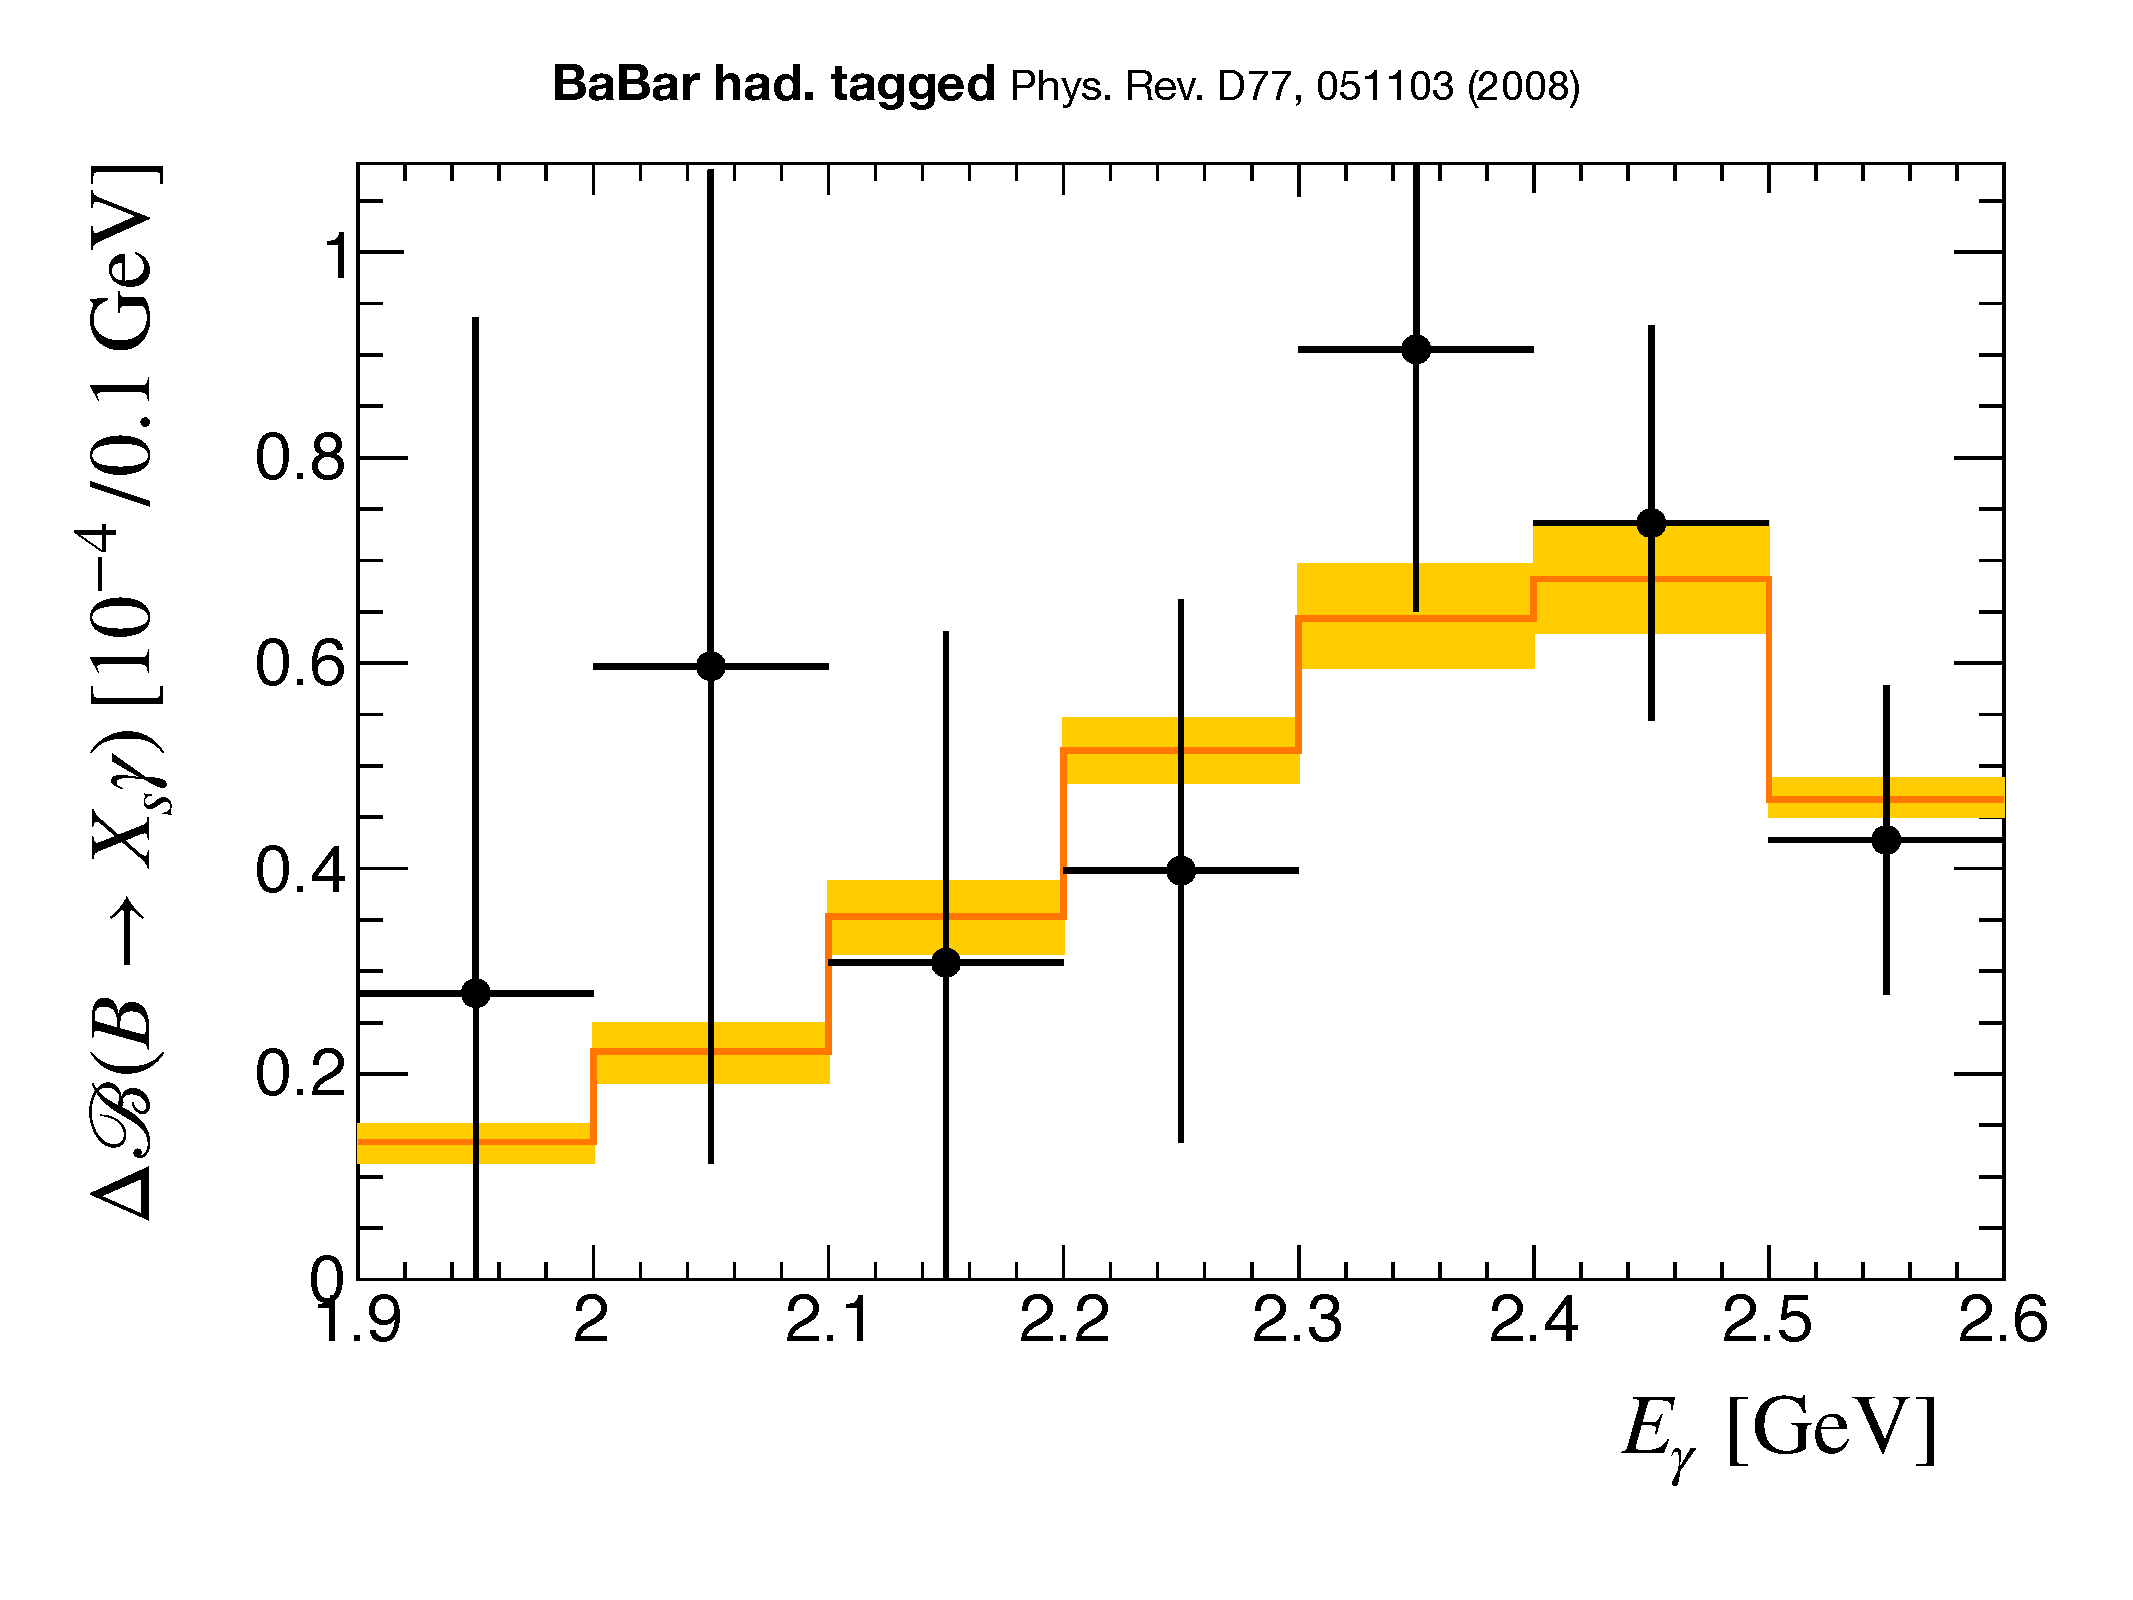
\includegraphics[width=0.7\textwidth]{figures/babar_hadtag_spec_default_la055_a3.pdf}
         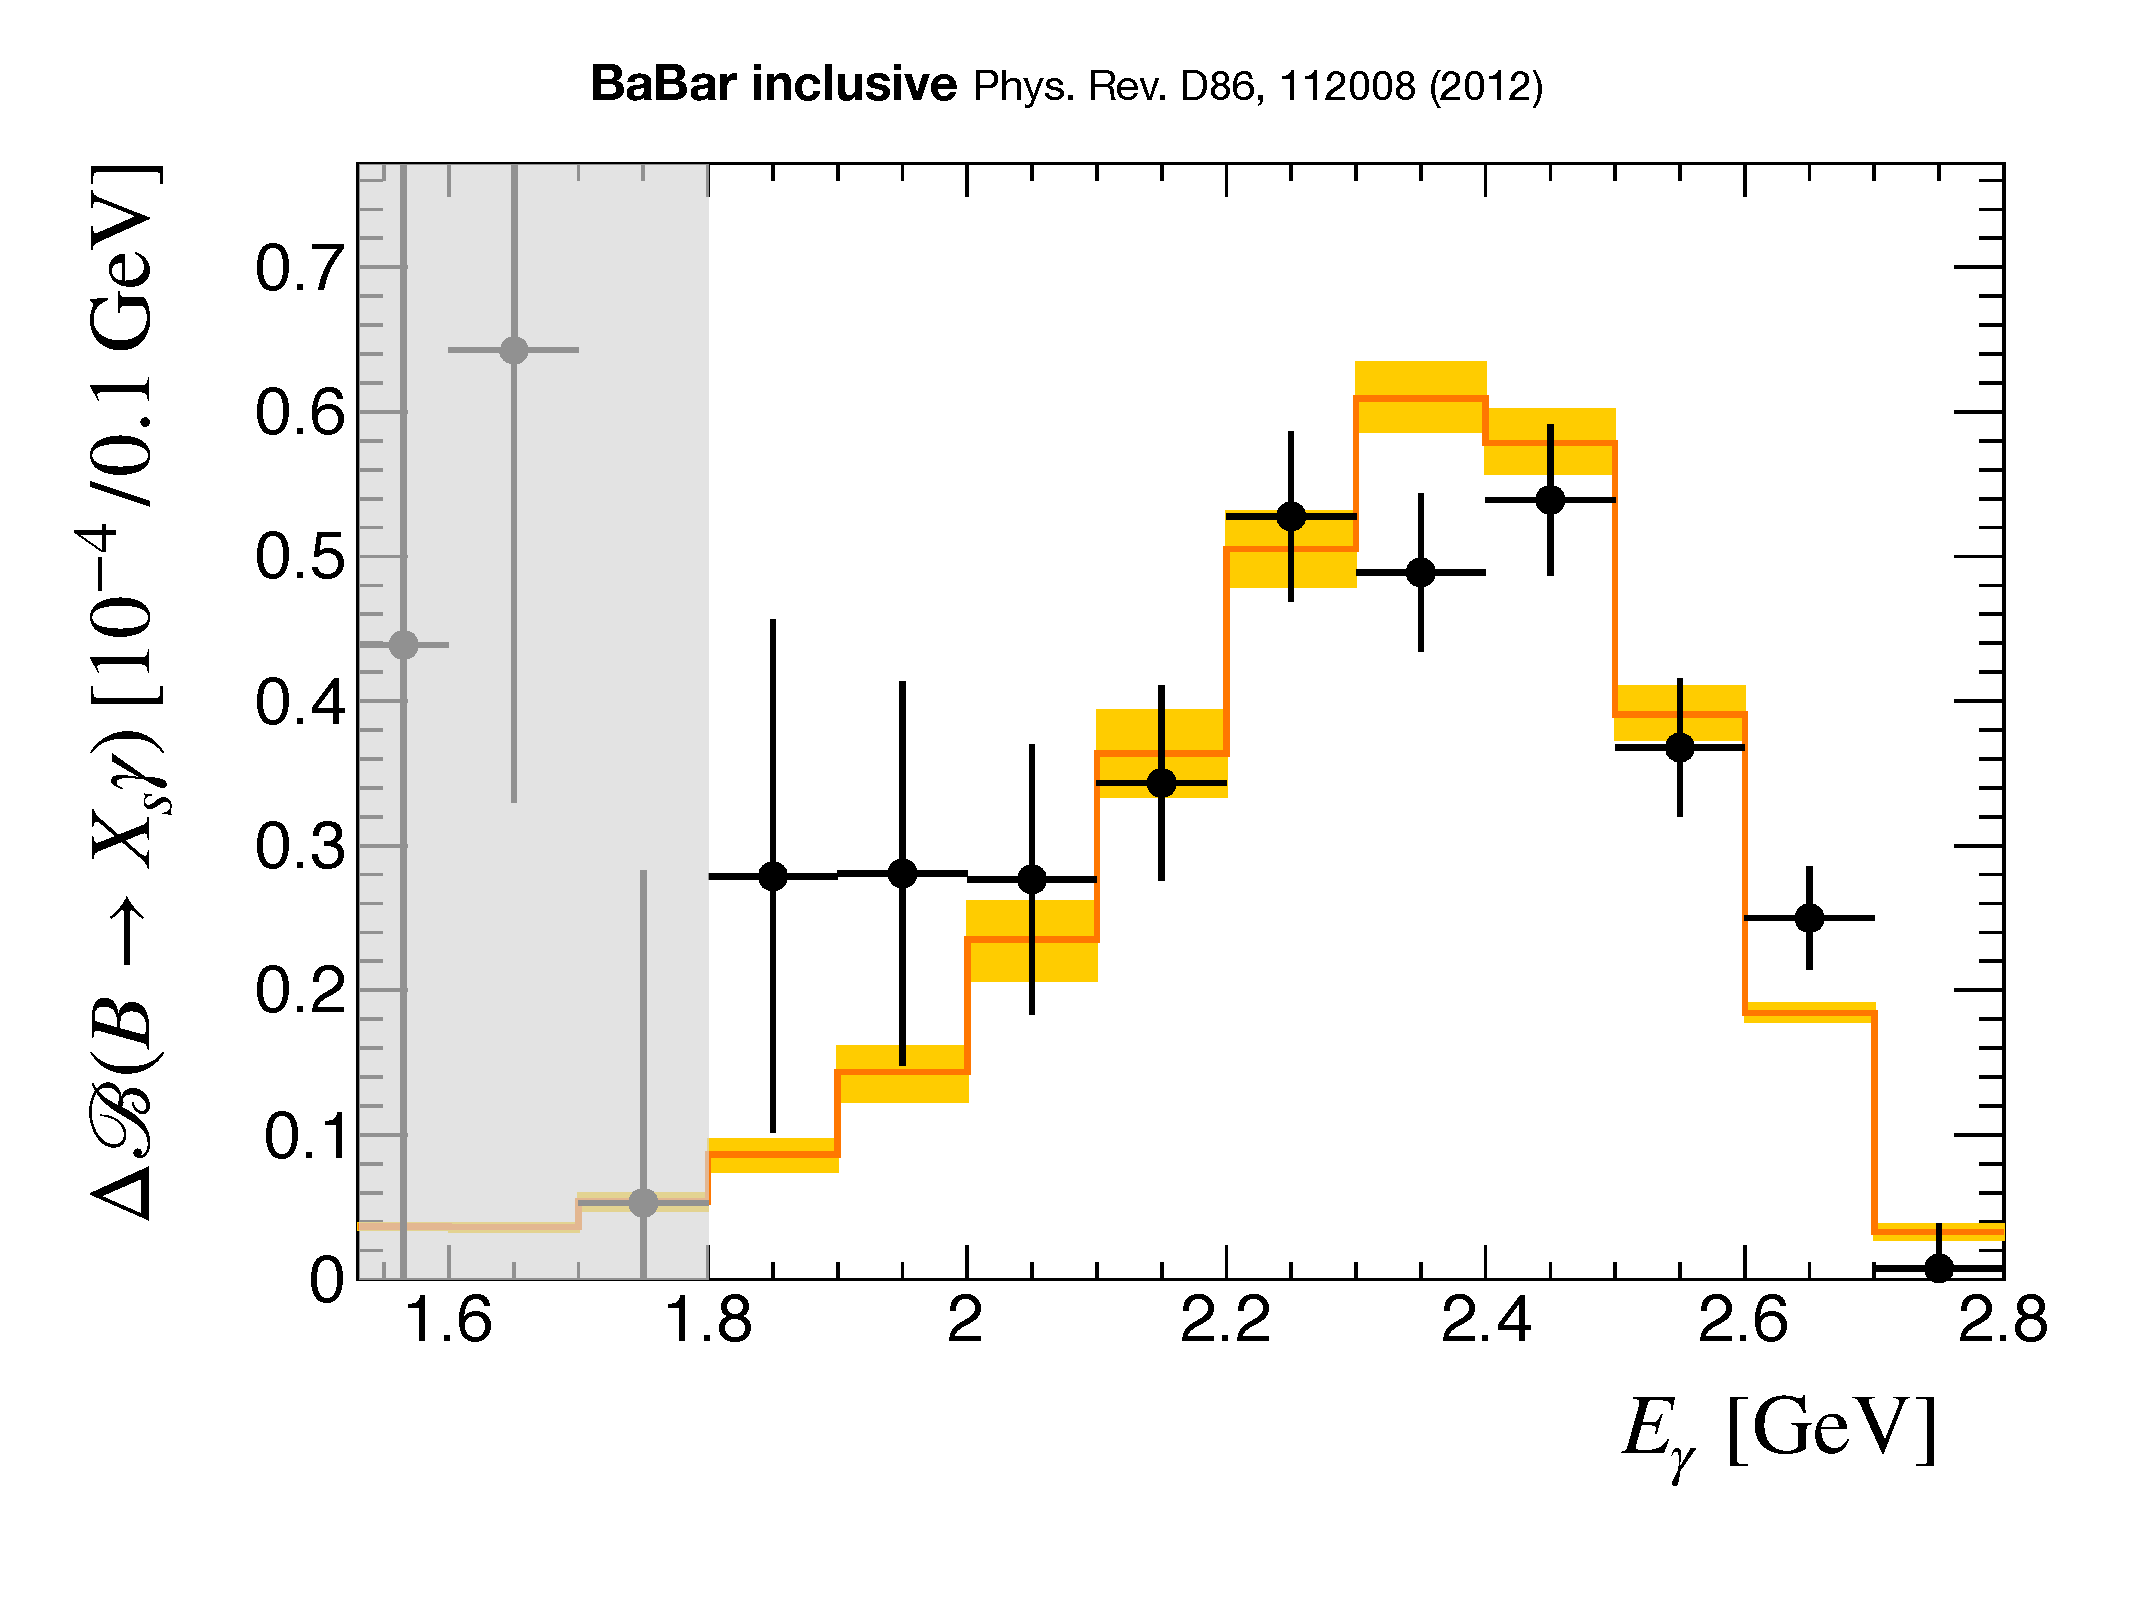
\includegraphics[width=0.7\textwidth]{figures/babar_incl_spec_default_la055_a3.pdf}
         \column{0.5\textwidth}
         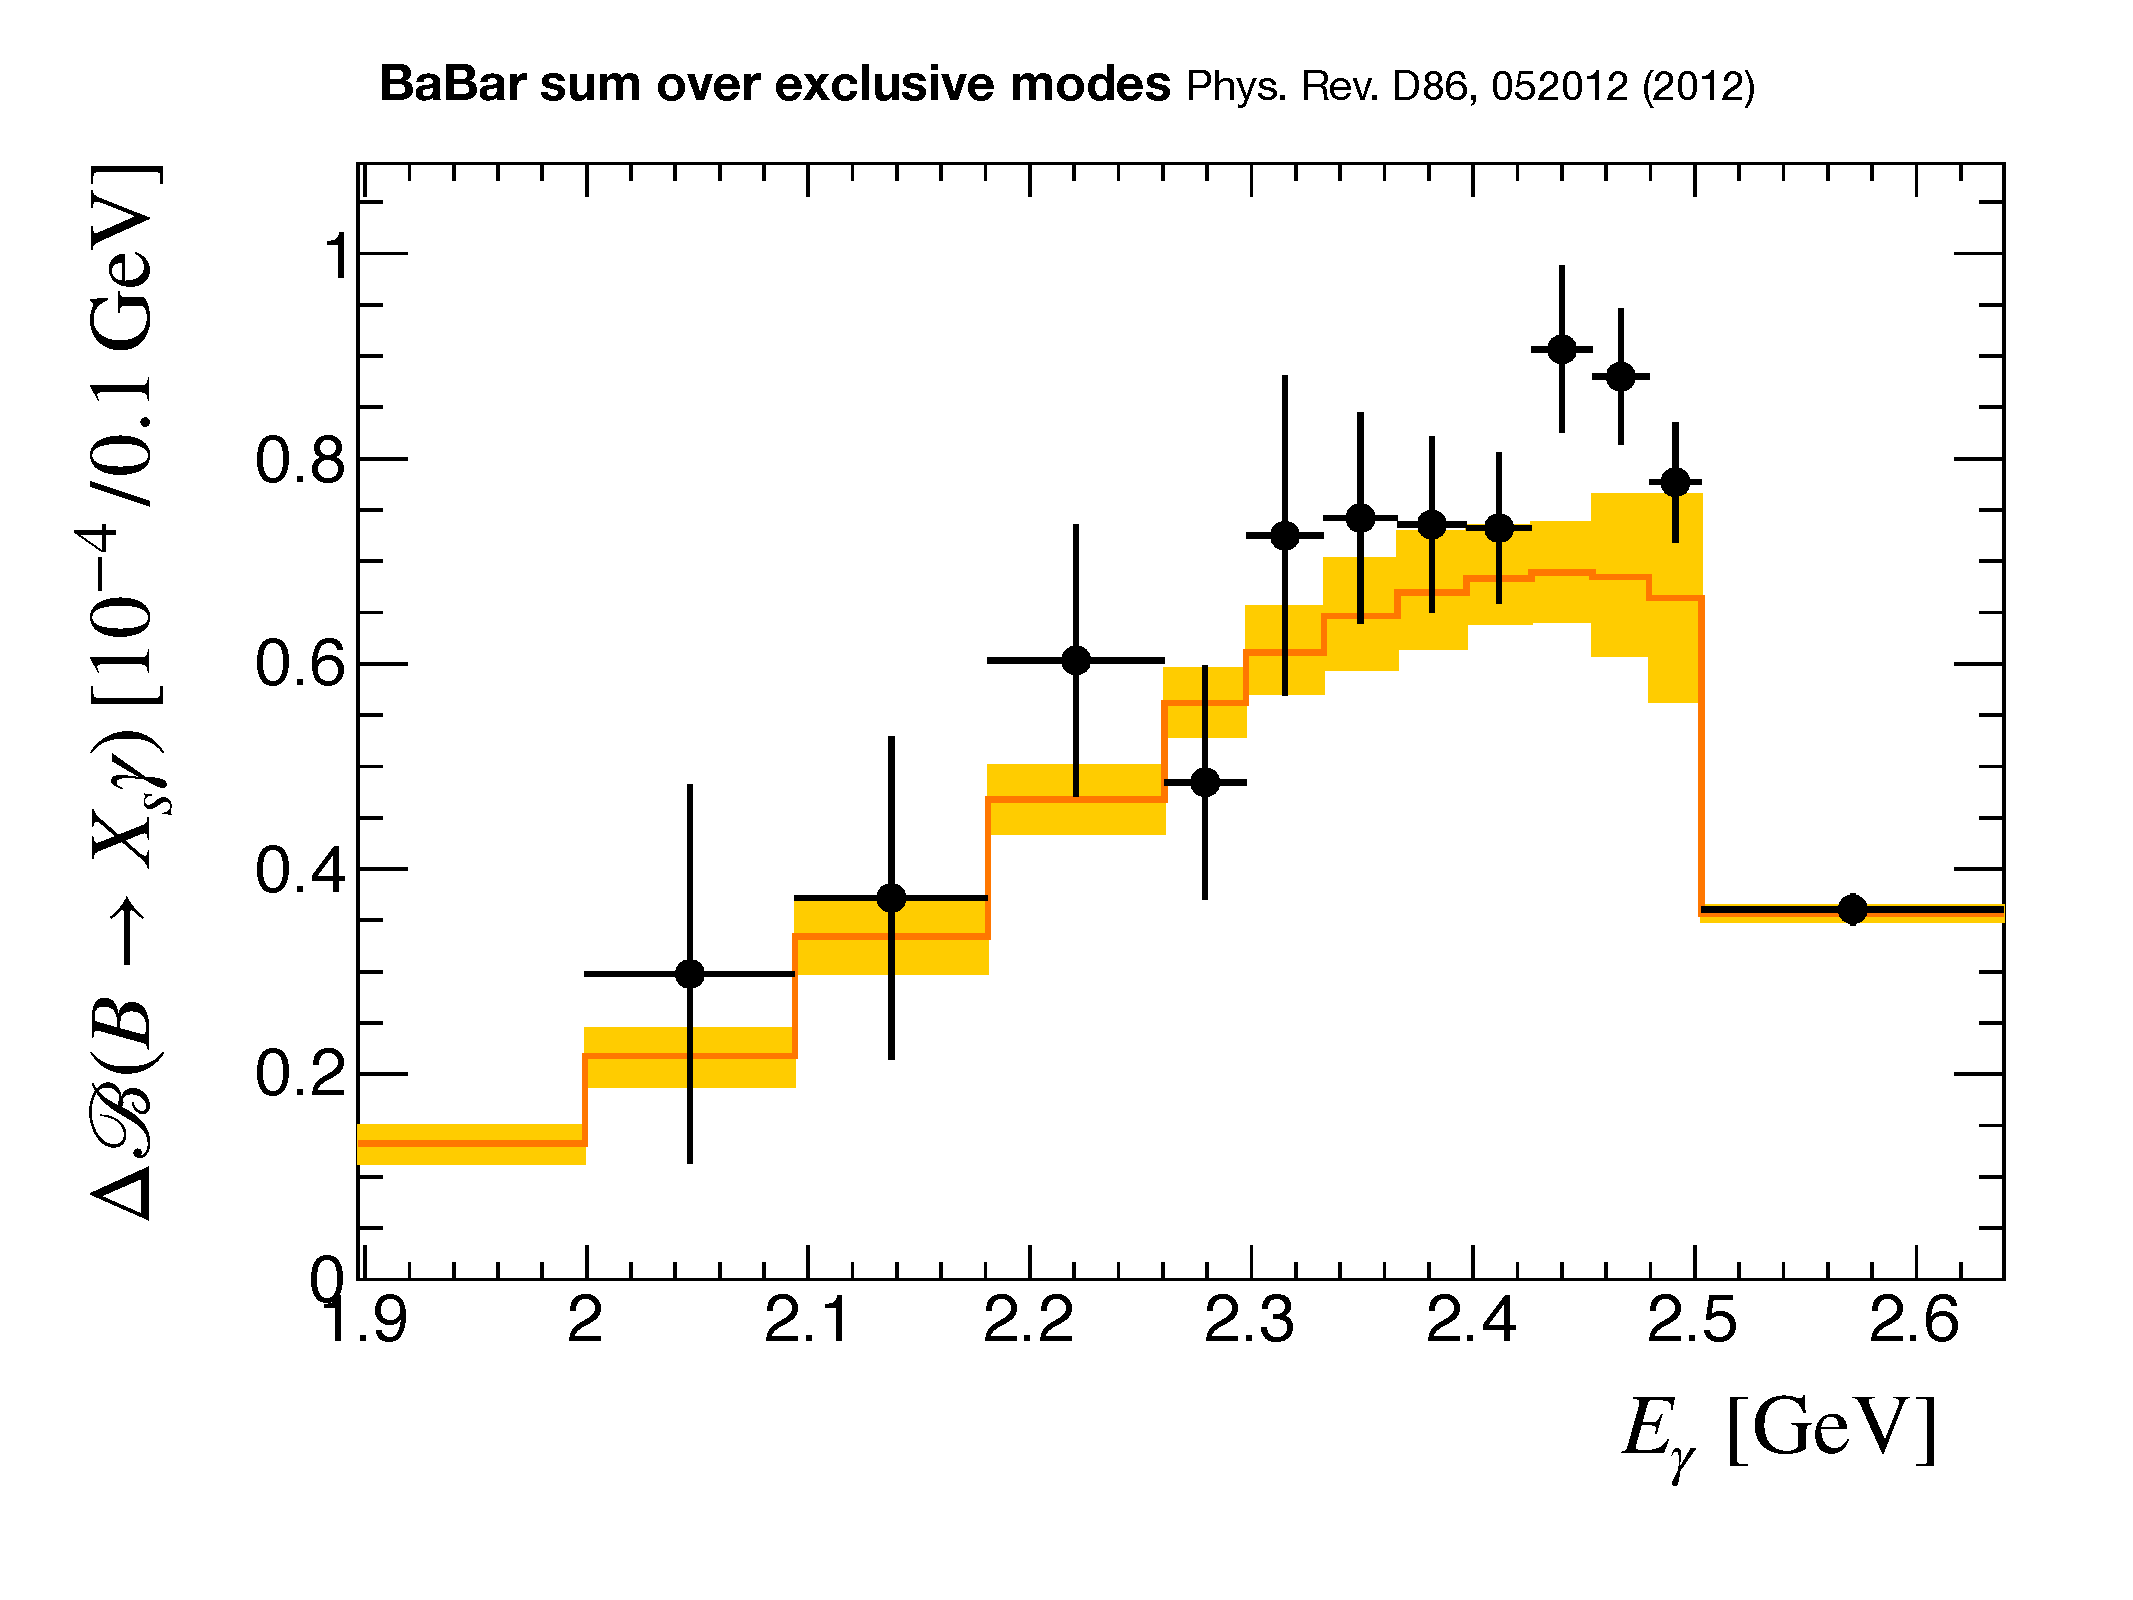
\includegraphics[width=0.7\textwidth]{figures/babar_sem_spec_default_la055_a3.pdf}
         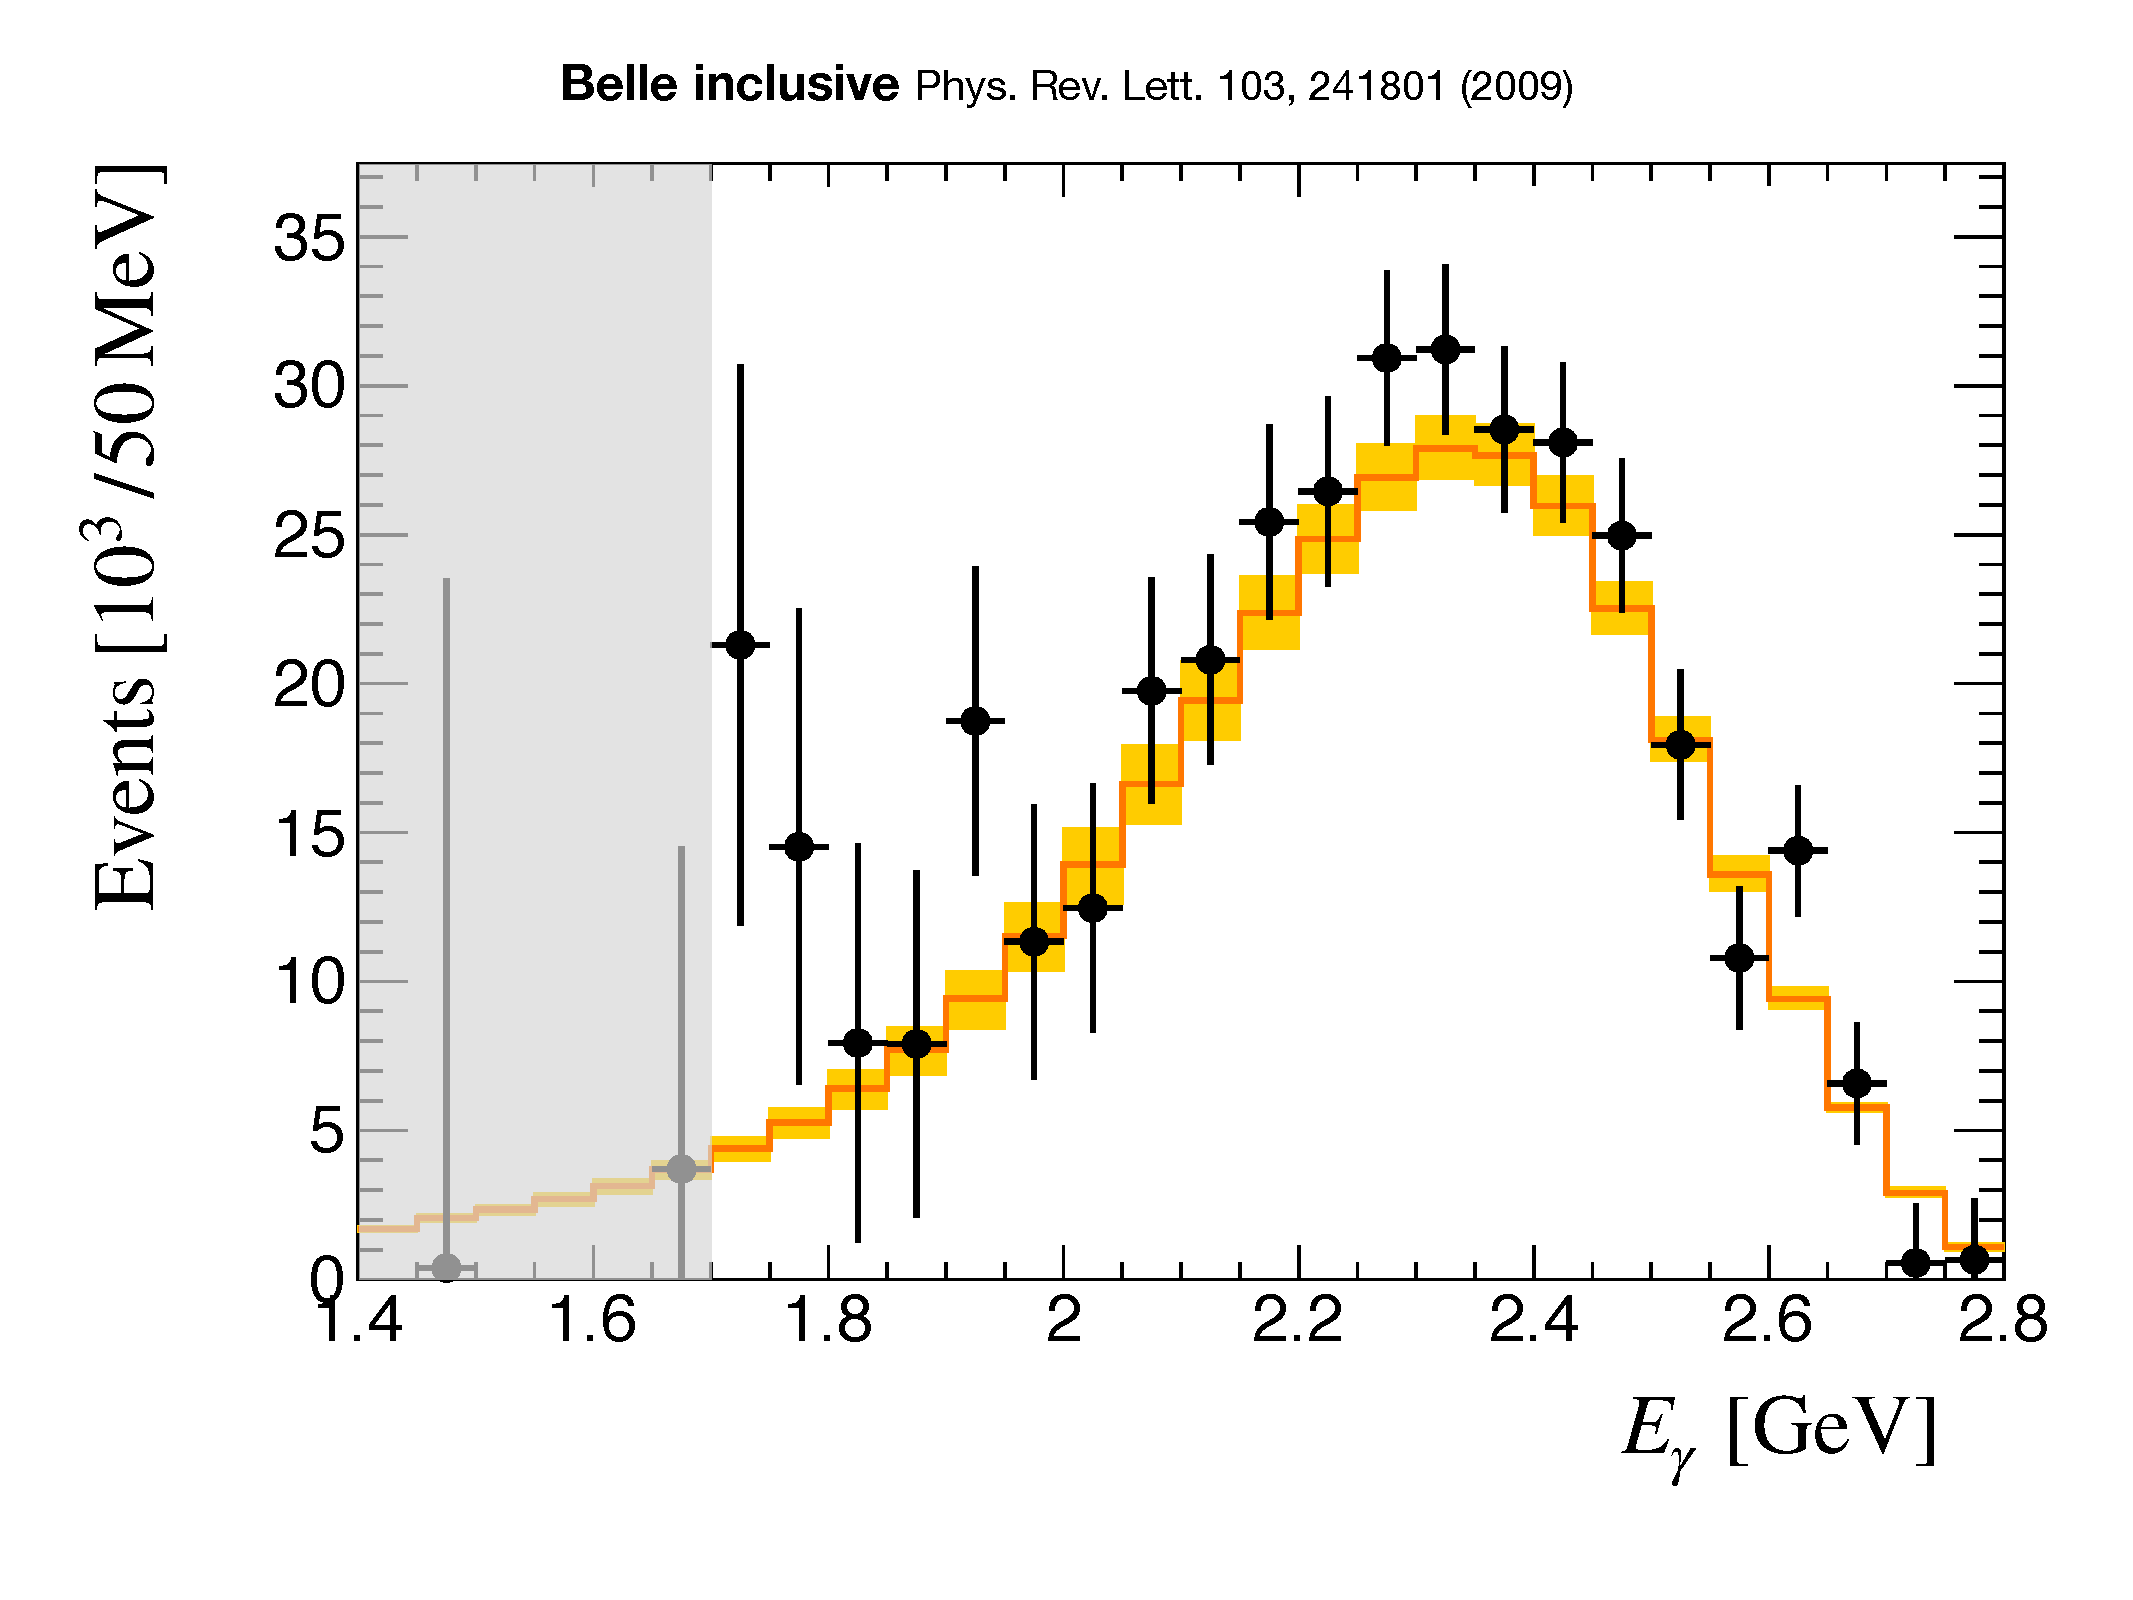
\includegraphics[width=0.7\textwidth]{figures/belle_spec_default_la055_a3.pdf}
      \end{columns}
      \begin{flushright}
         {\tiny\textbf{Phys.Rev.Lett. 127 (2021) 10, 102001}}
      \end{flushright}
   \end{frame}

\begin{frame}{Beyond the Standard Model}
   \small
   Only heavy particles are expected, in other words, the effective Lagrangian would be modified as:
   \begin{equation}\nonumber
      \mathcal{C}_i^{\mathrm{SM}} \ra \mathcal{C}_i^{\mathrm{SM}} + \Delta\mathcal{C}_i^{\mathrm{BSM}}.
   \end{equation}
   Some models may propose $\Delta\mathcal{C}_j^{\mathrm{BSM}}$, where $\mathcal{C}_j^{\mathrm{SM}}=0$

\vspace{10pt}
   In no particular order, some (but surely not all) theories which propose such modifications:
   \begin{itemize}
      \item two-Higgs-doublet models $\leftarrow$ \textbf{to my knowledge, the most studied}
      \item minimal supersymmetric models with minimal flavour violation
      \item and left-right symmetric models
      \item general minimal-supersymmetric theories
      \item models with extra dimensions
      \item the littlest Higgs models
      \item 331 models
   \end{itemize}
\end{frame}

   %----------------------------------------------------------------------------------------
   %	Experimental status
   %----------------------------------------------------------------------------------------
   \section{\safeBtoXsdgamma experimental status}

   \begin{frame}{\safeBtoXsgamma experimental status}
      \small
      \begin{equation}\nonumber
         \mathcal{B}(\BtoXsgamma) = (3.40\pm 0.17) \cdot 10 ^{-4}
      \end{equation}

      whereas the experimental value is:

      \begin{equation}\nonumber
         \mathcal{B}(\BtoXsgamma) = (3.49\pm 0.19) \cdot 10 ^{-4}
      \end{equation}

      which is a combination of the following measurements:
      \vspace{5pt}

      \resizebox{1.\textwidth}{!}{
         \begin{tabular}{|lllllc|}
         \hline
         Year & Experiment                 & Technique & Data used  & Energy threshold &  $\mathcal{B}(B\rightarrow X_s\gamma) \times 10^{-4}$  [$\EB>1.6~\gev$]\\ 
         \hline
         2001 & CLEO   & Untagged         & 9.1~\invfb &  $\EB>2.0~\gev$ & $3.29\pm0.44\pm0.29$\\ 
         2007 & BaBar & Hadronic-tagged  & 210~\invfb &  $\EB>1.9~\gev$ & $3.90\pm0.91\pm0.64$\\ 
         2009 & Belle & Untagged/Lepton-tagged      & 605~\invfb &  $\EB>1.7~\gev$ & $3.47\pm0.15\pm0.40$\\ 
         2012 & BaBar  & Lepton-tagged         & 347~\invfb &  $\EB>1.7~\gev$ & $3.32\pm0.16\pm0.31$\\ 
         2012 & BaBar  & Sum-of-exclusive & 429~\invfb &  $\EB>1.7~\gev$ & $3.52\pm0.20\pm0.51$\\ 
         2014 & Belle & Sum-of-exclusive & 711~\invfb &  $\EB>1.7~\gev$ & $3.75\pm0.18\pm0.35$\\
         %\hline
         %2022 & {\bf Belle II}& Hadronic               & 189 fb$^{-1}$ & $3.54 \pm0.78 (\mathrm{stat.})\pm0.83(\mathrm{syst.})$ &              $E^B_{\gamma}>1.8~\gev$                 \\
         \hline
         \end{tabular}
         }
         
         \vspace{10pt}

         Notice three prevalent type of measurement techniques:
         \begin{itemize}
            \item Sum-of-exclusive
            \item Untagged
            \item Tagged
         \end{itemize}
         \textbf{Only obtained by $\bm{B}$ factories}!
   \end{frame}

   \begin{frame}{\safeBtoXsgamma measurement techniques}
      \begin{columns}
         \centering
         \column{0.4\textwidth}
         \pgfdeclarelayer{bg}    % declare background layer
\pgfsetlayers{bg,main}  % set the order of the layers (main is the standard layer)
\begin{tikzpicture}[rotate=90]

    % NODES
    
    % Initial state
    \node [circle, minimum size=1.2cm, draw=white, ultra thick]    (collision) {} ;
    % \node [] (collision) {} ;
    \node [] (collisiontext) [below=0.03cm of collision.west] {\FourS};
    \node [] (eminus)     [left=2cm of collision.center] {};
    \node [] (eplus)     [right=1.5cm of collision.center] {};
    \node [] (eplusabove) [above=0.1cm of eplus] {};
    \node [] (eminusabove) [above=0.1cm of eminus] {};
    \node [] (eminustext)     [right=0.3cm of eminusabove, text=blue] {\en};
    \node [] (eplustext)     [left=0.3cm of eplusabove, text=red] {\ep};
    
    % BB bar
    \node [] (bbarup) [above=0.7cm of collision.north east] {};
    \node [] (bbardown) [below=0.5cm of collision.south east] {};
    \node [] (bbarup_text) [right=0.05cm of bbarup.center] {$\B_{\mathrm{sig}}$};
    \node [] (bbardown_text) [right=0.05cm of bbardown.center] {$\B_{\mathrm{tag}}$};
    
    % Xs gamma
    %%gamma
    \node [] (gamma_int) [left=0.5cm of bbarup.center] {};
    \node [] (gamma) [above=1cm of gamma_int.center] {};
    \node [] (gammatext) [left=0.05cm of gamma.center] {$\gamma$};
    %%xs
    \node [] (Xs_int) [right=0.5cm of bbarup.center] {};
    \node [] (Xs) [above=0.5cm of Xs_int.center] {};
    \node [] (Xstext) [left=0.05cm of Xs.center] {$X_{s}$};
    %%xs daughters
    \node [] (Xsd1_int) [left=0.05cm of Xs.center] {};
    \node [] (Xsd1) [above=0.5cm of Xsd1_int.center] {};
    \node [] (Xsd2_int) [right=0.2cm of Xs.center] {};
    \node [] (Xsd2) [above=0.4cm of Xsd2_int.center] {};
    \node [] (Xsd3_int) [right=0.35cm of Xs.center] {};
    \node [] (Xsd3) [above=0.2cm of Xsd3_int.center] {};
    
    % Tag side
    
    % first generation
    \node [] (D0_int) [left=0.35cm of bbardown.center] {};
    \node [] (D0) [below=0.65cm of D0_int.center] {};
    \node [] (pi0_int) [right=0.3cm of bbardown.center] {};
    \node [] (pi0) [below=0.6cm of pi0_int.center] {};
    
    %second generation
    \node [] (Kp_int) [left=0.25cm of D0.center] {};
    \node [] (Kp) [below=0.65cm of Kp_int.center] {};
    \node [] (pim_int) [right=0.1cm of D0.center] {};
    \node [] (pim) [below=0.6cm of pim_int.center] {};

    \node [] (g1_int) [left=0.2cm of pi0.center] {};
    \node [] (g1) [below=0.65cm of g1_int.center] {};
    \node [] (g2_int) [right=0.15cm of pi0.center] {};
    \node [] (g2) [below=0.6cm of g2_int.center] {};
    
    %\node [] (hadron text) [below=0.05cm of bbardown.center] {\scriptsize hadrons};
    
    % Colored overal blocks
    
    \node [] (sigside) [above=0.8cm of bbarup] {};
    \node [] (tagside) [below=0.8cm of bbardown] {};
    \node [] (tagside_right) [right=0.2cm of tagside] {};
    
    \node [] (sigsidetext) [above=0.1cm of sigside] {\scriptsize Signal side};
    \node [] (tagsidetext) [below=0.3cm of tagside_right, text width = 2cm] {\centering\scriptsize Tag side};
    
    \begin{pgfonlayer}{bg}    % select the background layer
    \node [rectangle, fill=green!20, text width=2cm, text centered, rounded corners, minimum height=1.7cm] (Signal_Side) at (sigside) {};
    \node [rectangle, fill=blue!20, text width=2cm, text centered, rounded corners, minimum height=1.7cm] (Signal_Side) at (tagside) {};
    \end{pgfonlayer}

    

    
    % LINES
    
    % Initial state
    \draw [-Triangle, blue, thick] (eminus) -- (collision.center);
    \draw [-Triangle, red, thick] (eplus) -- (collision.center);
    
    % BB bar
    \draw[-Triangle, thick] (collision.center) -- (bbarup.center);
    \draw[-Triangle, thick] (collision.center) -- (bbardown.center);
    
    % Xs gamma
    \draw[-Triangle, thick, purple, dashed] (bbarup.center) -- (gamma.center);
    \draw[-Triangle, thick] (bbarup.center) -- (Xs.center);
    \draw[-Triangle, thick] (Xs.center) -- (Xsd1.center);
    \draw[-Triangle, thick] (Xs.center) -- (Xsd3.center);
    \draw[-Triangle, thick] (Xs.center) -- (Xsd2.center);
    
    % Tag side
    \draw[-Triangle, thick] (bbardown.center) -- (D0.center);
    \draw[-Triangle, thick] (bbardown.center) -- (pi0.center);

    \draw[-Triangle, thick] (D0.center) -- (Kp.center);
    \draw[-Triangle, thick] (D0.center) -- (pim.center);
    \draw[-Triangle, thick, dashed] (pi0.center) -- (g1.center);
    \draw[-Triangle, thick, dashed] (pi0.center) -- (g2.center);
    

    
\end{tikzpicture}
         \column{0.6\textwidth}
         \centering
         \textbf{Sum of exclusive}
         \begin{itemize}
            \item Reconstruct specific $X_s$ states:
            \begin{itemize}
               \item $K^*(892)$
               \item $K^+p^-$\\
               etc.
            \end{itemize} 
            \item Sum all reconstructed states
            \item Correct for missing phase space using simulation
         \end{itemize}

         Very efficient!

         But strongly simulation dependent...


      \end{columns}
   \end{frame}

   \begin{frame}{\safeBtoXsgamma measurement techniques}
      \begin{columns}
         \centering
         \column{0.4\textwidth}
         \pgfdeclarelayer{bg}    % declare background layer
\pgfsetlayers{bg,main}  % set the order of the layers (main is the standard layer)
\begin{tikzpicture}[rotate=90]

    % NODES
    
    % Initial state
    \node [circle, minimum size=1.2cm, draw=white, ultra thick]    (collision) {} ;
    % \node [] (collision) {} ;
    \node [] (collisiontext) [below=0.03cm of collision.west] {\FourS};
    \node [] (eminus)     [left=2cm of collision.center] {};
    \node [] (eplus)     [right=1.5cm of collision.center] {};
    \node [] (eplusabove) [above=0.1cm of eplus] {};
    \node [] (eminusabove) [above=0.1cm of eminus] {};
    \node [] (eminustext)     [right=0.3cm of eminusabove, text=blue] {\en};
    \node [] (eplustext)     [left=0.3cm of eplusabove, text=red] {\ep};
    
    % BB bar
    \node [] (bbarup) [above=0.7cm of collision.north east] {};
    \node [] (bbardown) [below=0.5cm of collision.south east] {};
    \node [] (bbarup_text) [right=0.05cm of bbarup.center] {$\B_{\mathrm{sig}}$};
    \node [] (bbardown_text) [right=0.05cm of bbardown.center] {$\B_{\mathrm{tag}}$};
    
    % Xs gamma
    %%gamma
    \node [] (gamma_int) [left=0.5cm of bbarup.center] {};
    \node [] (gamma) [above=1cm of gamma_int.center] {};
    \node [] (gammatext) [left=0.05cm of gamma.center] {$\gamma$};
    %%xs
    \node [] (Xs_int) [right=0.5cm of bbarup.center] {};
    \node [] (Xs) [above=0.5cm of Xs_int.center] {};
    \node [] (Xstext) [left=0.05cm of Xs.center] {$X_{s}$};
    %%xs daughters
    \node [] (Xsd1_int) [left=0.05cm of Xs.center] {};
    \node [] (Xsd1) [above=0.5cm of Xsd1_int.center] {};
    \node [] (Xsd2_int) [right=0.2cm of Xs.center] {};
    \node [] (Xsd2) [above=0.4cm of Xsd2_int.center] {};
    \node [] (Xsd3_int) [right=0.35cm of Xs.center] {};
    \node [] (Xsd3) [above=0.2cm of Xsd3_int.center] {};
    
    % Tag side
    
    % first generation
    \node [] (D0_int) [left=0.35cm of bbardown.center] {};
    \node [] (D0) [below=0.65cm of D0_int.center] {};
    \node [] (pi0_int) [right=0.3cm of bbardown.center] {};
    \node [] (pi0) [below=0.6cm of pi0_int.center] {};
    
    %second generation
    \node [] (Kp_int) [left=0.25cm of D0.center] {};
    \node [] (Kp) [below=0.65cm of Kp_int.center] {};
    \node [] (pim_int) [right=0.1cm of D0.center] {};
    \node [] (pim) [below=0.6cm of pim_int.center] {};

    \node [] (g1_int) [left=0.2cm of pi0.center] {};
    \node [] (g1) [below=0.65cm of g1_int.center] {};
    \node [] (g2_int) [right=0.15cm of pi0.center] {};
    \node [] (g2) [below=0.6cm of g2_int.center] {};
    
    %\node [] (hadron text) [below=0.05cm of bbardown.center] {\scriptsize hadrons};
    
    % Colored overal blocks
    
    \node [] (sigside) [above=0.8cm of bbarup] {};
    \node [] (tagside) [below=0.8cm of bbardown] {};
    \node [] (tagside_right) [right=0.2cm of tagside] {};
    
    \node [] (sigsidetext) [above=0.1cm of sigside] {\scriptsize Signal side};
    \node [] (tagsidetext) [below=0.3cm of tagside_right, text width = 2cm] {\centering\scriptsize Tag side};
    
    \begin{pgfonlayer}{bg}    % select the background layer
    \node [rectangle, fill=green!20, text width=2cm, text centered, rounded corners, minimum height=1.7cm] (Signal_Side) at (sigside) {};
    \node [rectangle, fill=blue!20, text width=2cm, text centered, rounded corners, minimum height=1.7cm] (Signal_Side) at (tagside) {};
    \end{pgfonlayer}

    

    
    % LINES
    
    % Initial state
    \draw [-Triangle, blue, thick] (eminus) -- (collision.center);
    \draw [-Triangle, red, thick] (eplus) -- (collision.center);
    
    % BB bar
    \draw[-Triangle, thick] (collision.center) -- (bbarup.center);
    \draw[-Triangle, thick] (collision.center) -- (bbardown.center);
    
    % Xs gamma
    \draw[-Triangle, thick, purple, dashed] (bbarup.center) -- (gamma.center);
    \draw[-Triangle, thick] (bbarup.center) -- (Xs.center);
    \draw[-Triangle, thick] (Xs.center) -- (Xsd1.center);
    \draw[-Triangle, thick] (Xs.center) -- (Xsd3.center);
    \draw[-Triangle, thick] (Xs.center) -- (Xsd2.center);
    
    % Tag side
    \draw[-Triangle, thick] (bbardown.center) -- (D0.center);
    \draw[-Triangle, thick] (bbardown.center) -- (pi0.center);

    \draw[-Triangle, thick] (D0.center) -- (Kp.center);
    \draw[-Triangle, thick] (D0.center) -- (pim.center);
    \draw[-Triangle, thick, dashed] (pi0.center) -- (g1.center);
    \draw[-Triangle, thick, dashed] (pi0.center) -- (g2.center);
    

    
\end{tikzpicture}
         \column{0.6\textwidth}
         \centering
         \textbf{Untagged/Tagged}

         \begin{itemize}
            \item Do not reconstruct $X_s$: treat them in a `missing-momentum' way
            \item Suppress background only using the information of the photon
            \item \textbf{If tagging}: also use the information of the second $B$ meson
         \end{itemize}

         \begin{tikzpicture}
            \node[anchor = south west, inner sep=0] (image) at (current page.south west) 
                {\includegraphics[width=0.8\textwidth]{../phd_thesis/figures/experiment_overview/tagging_advantages_mod.png}};
            \node[below = 5 mm of image] (ghost) {};
               \node[align = center, left =15mm of ghost] (firsttext)% <---- 
                {\footnotesize \textbf{Untagged}};
            \node[right = 2 mm of firsttext] (temp) {};
            \node[align = center, above = 1mm of temp] (secondtext)% <---- 
                {\footnotesize \textbf{lepton tagging}};
            \node[align = center, right = 6mm of firsttext] (thirdtext)% <---- 
                {\footnotesize \textbf{semileptonic tagging}};
            \node[align = center, right = 6mm of secondtext] (fourthtext)% <---- 
                {\footnotesize \textbf{hadronic tagging}};
         \end{tikzpicture}
      \end{columns}
   \end{frame}

   %----------------------------------------------------------------------------------------
   %	Belle II
   %----------------------------------------------------------------------------------------
   \section{Belle~II and SuperKEKB}

   \begin{frame}{Belle~II and SuperKEKB}
   \end{frame}


\end{document}
